\chapter{Grant-Free Access via Blind Signal Recovery using Wirtinger Flow}
\label{wfcma:chap}

In the first part of this dissertation, we focus on blind signal recovery methods to enable grant-free access in large scale networks.
We adopt recent results in non-convex optimization and leverage a geometric analysis of the blind signal recovery problem with limited data samples. This approach demonstrates that these non-convex problems enjoy a rather benign geometry and can be solved with relative ease. Moreover, it also allows us to formulate theoretical guarantees, ensuring convergence with high probability. \crfootnote{Part of this chapter is reprinted, with permission, from [C. Feres and Z. Ding, ``Wirtinger Flow Meets Constant Modulus Algorithm: Revisiting Signal Recovery for Grant-Free Access" in \textit{IEEE Transactions on Signal Processing (Early Access)}, Aug. 2021] and followup modifications for final publication. Notations may have changed for consistency throughout this dissertation.} 

In this chapter, we consider a prominent non-convex algorithm known as Wirtinger Flow (WF), which has shown strong results in related nonconvex problems in the literature. 
Due to the strong similarity between CMA-based signal recovery and the phase retrieval problem  \cite{Candes2015a_phaseretrievalWF}, we adopt the WF algorithm directly in CMA-based blind signal recovery, which we denote WF-CMA. 
In light of the convergence properties of WF under limited data samples, we leverage and generalize the original convergence analysis of WF in phase retrieval and obtain theoretical convergence guarantees for CMA in a finite-sample regime, both for single and multiple source recovery \cite{Feres2021WFCMA}.



%We demonstrate that the WF algorithm in the context of CMA is in fact a generalization of the phase retrieval problem that has recently gathered a lot of interest \cite{Candes2015a_phaseretrievalWF,Candes2013}. 
%In fact, we can formulate the CM minimization as Phase Retrieval based on mean amplitude information.  
%Another interesting observation is that the WF algorithm for CM cost minimization in fact coincides with the previously proposed ``normalized'' CMA or NCMA. 
%The convergence properties of NCMA have only been addressed via simulation examples. 
%Our major contribution lies in the analysis of WF to clearly characterize the convergence conditions of WF-based CMA and identify explicit choices of the iteration stepsize. 







\section{CMA-based Blind Signal Recovery}\label{wfcma:SystemModel}
Figure~\ref{wfcma:fig:system_model} depicts a blind signal recovery system at the base station. As presented in Section~\ref{system:ssec:blind_recovery}, such a system attempts to find a demixer $\bm{w}$ that recovers one of the transmitted signals with minimal interference, or more generally, to find $J$ demixers $\bm{w}_\ell$, $\ell\in\{1,\cdots,J\}$ that recover $J$ distinct source signals with minimal mutual interference.
{\begin{figure}[tbp]
		\centering
		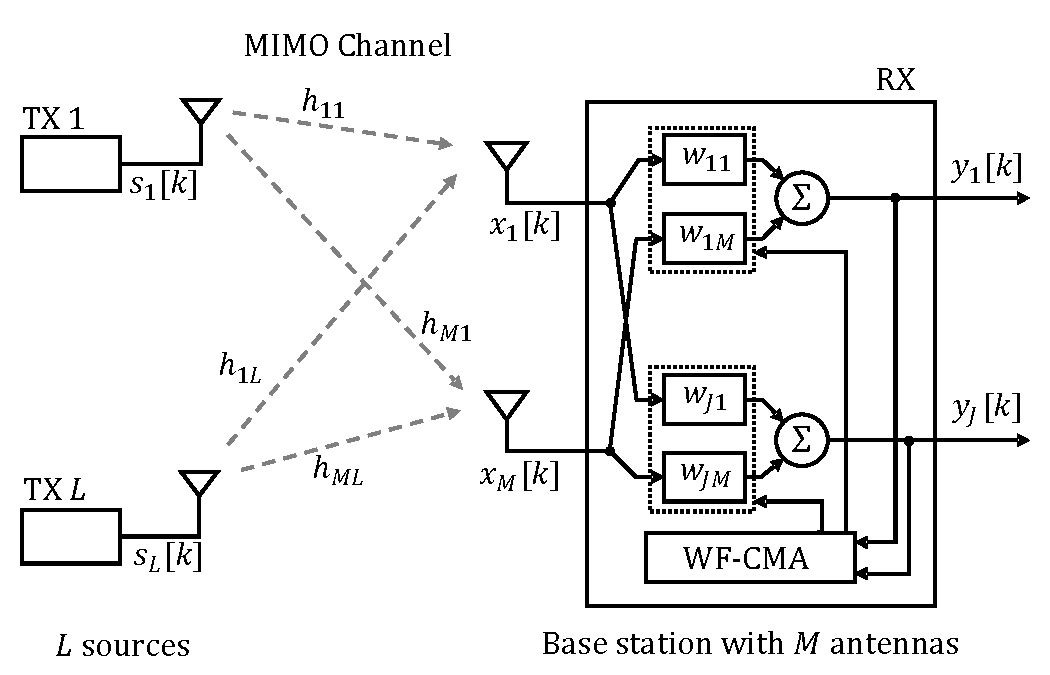
\includegraphics[width=0.6\linewidth]{./figs/wfcma_figs/WF-CMA_system_model.pdf}
		\caption{$L$ sources share a common resource block and transmit independent signals to a host station with $M$ antennas through an unknown physical channel. The host receiver aims to find multiple adaptive linear demixers $\bm{w}_1,\ldots,\bm{w}_J$ to recover $J\leq L$ sources with little mutual interference.}\label{wfcma:fig:system_model}
\end{figure}}

\subsection{Single Source Recovery}
Recall from Section~\ref{system:ssec:blind_recovery} the constant-modulus cost function proposed by Godard \cite{Godard1980cma}:
\begin{align}
	f(\w)=\displaystyle{\frac{1}{2K}\sum_{k=1}^K\Big(|\xk\herm\w|^2-R_2\Big)^2},\label{wfcma:eqn:cma_orig}
\end{align}
where $R_2$ is defined as in Eq.(\ref{system:eqn:cma_ssr_expectation}), but can be set to any value (e.g. $R_2=1$) and will scale the magnitude of the demixer $\bm{w}$ accordingly. As stated in Section~\ref{system:ssec:blind_recovery}, we assume that all sources have equal average energy, as different signal energies can be considered as a channel effect. Additionally, recall that the base station does not know the active number of sources $L$, and we only assume that $L\leq M$ to ensure a full-column rank channel.

The CM cost function \ref{wfcma:eqn:cma_orig} has been proven to converge in expectation under noiseless scenarios and full-column rank channel \cite{Ding2000,LiDing1994cmaglobalconvergencefse}. Nevertheless, to the best of our knowledge there were no convergence guarantees under limited data samples in the literature previous to this work. This is one of the main results we present later in this chapter, and we further make use of this result to prove convergence in the multiple source recovery setting. 

\subsection{Regularization for Multiple Signal Recovery}

As we assume that multiple devices may access the channel in a grant-free scenario, it is desirable to recover  multiple source signals at a time as described in Section~\ref{system:ssec:blind_recovery}. If we attempt to simultaneously recover multiple sources by solving for multiple demixer vectors $\bm{w}_{\ell}\in\{1\ldots,J\}$, we need to ensure that they do not restore the same source signal, possibly with different phases or delays \cite{Ding2000}. 

Therefore, additional adjustments must be considered. Now, given that the different sources are independent, this is equivalent to force statistical uncorrelatedness of the signals in the cost function. 
For the case of complex outputs $y_{\ell},y_{i}$, their covariance is given by:
\begin{align}
\mathrm{Cov}\{y_{i},y_{\ell}\}
&=\mathbb{E}\{y_{i}y_{\ell}^*\}
=\mathbb{E}\{\w_{i}\herm\bm{x_k}(\w_{\ell}\herm\bm{x_k})^*\}
%\nonumber\\&
=\w_{i}\herm\mathbb{E}\{\xk\xk\herm\}\w_{\ell}.
\end{align}

Thus, we propose to regularize the CMA cost function with the squared magnitude of the pairwise covariances of the outputs, to obtain a smooth real-valued cost function. The modified CMA cost function for multiple sources considers $J$ copies of the CM cost function (\ref{wfcma:eqn:cma_orig}), each one depending on a different demixer, and our proposed regularization:
\begin{align}
&g(\w_1,\ldots,\w_J)=%\nonumber\\
%&\qquad\qquad
\sum_{\ell=1}^Jf(\w_\ell) +\gamma_0\sum_{\ell=1}^J\sum_{i\neq \ell}^J\big|\w_{i}\herm\bm{R}_{\bm{x}}\w_{\ell}\big|^2, \label{wfcma:eqn:cma_msr}
\end{align}
where $\gamma_0>0$ is a constant and the sample covariance matrix
\begin{align}
\bm{R}_{\bm{x}}=\frac{1}{K}\sum_{k=1}^K\xk\xk\herm.
\end{align}  

This is related to the regularization proposed in \cite{Chen1991crimno} which uses joint cumulants for source separation. The joint cumulants also consider the potential correlatedness of delayed versions of the demixer outputs, but in the presented case of source recovery the channels have no ISI, and the information from different delays of the outputs is not necessary. Other similar regularized approaches have been proposed in \cite{Bessios1992mimocrimno,Li1998adaptivemimocma}.


\section{WF-Based Constant Modulus Solutions} \label{wfcma:WF}

\subsection{CMA meets Wirtinger Flow} 

A recent stream of nonconvex optimization procedures have been developed for solving quadratic equations, in particular for the phase retrieval problem. The phase retrieval problem can be stated as the recovery of an unknown signal $\bm{z}$ using known sampling vectors $\bm{a}_k$ from magnitudes $r_k=|\bm{a}_k\herm \bm{z}|^2$ only for which the smooth cost function is
\begin{equation}
\min_{\bm{z}\in\mathbb{C}^M}\quad \frac{1}{2K}\sum_{k=1}^K\big(|\bm{a}_k\herm\bm{z}|^2-r_k\big)^2. \label{wfcma:eqn:phaseretrieval}
\end{equation}

Note that in terms of the cost functions, phase retrieval is equivalent to the single-source CMA problem in Eq.(\ref{wfcma:eqn:cma_orig}), by setting $r_k=R_2$ and $\bm{a_k}=\bm{x}_k$, $k\in\{1,\ldots,K\}$, and using $\bm{z}$ as the unknown variable. 
If the source signal has constant modulus, e.g., $|s_{\ell}[k]|^2=R_2$ for PSK signals, then the CM cost is the same as in the phase retrieval. 
One the other hand, for non-constant modulus source signals, e.g. 16-QAM, the CM cost is akin to phase retrieval based on an ``average magnitude''.

This similarity stimulates this study on the link between optimization methods for phase retrieval and the CMA problem. 
However, there are some fundamental differences: 
(A) In phase retrieval, there is a known reference signal $r_k$ as ground truth which is fully exploited in its convergence analysis. However, in CM-based demixing we only have a desired ``average magnitude'' $R_2$.  
(B) Phase retrieval has only one solution (up to common rotations), where in blind demixing, there may be many ideal demixer vectors to recover multiple source signals in different order (up to common rotations). 
(C) The sampling vectors $\bm{a}_k$ are chosen typically as Gaussian by users in phase retrieval. In CMA, $\bm{x}_k$ is (noisy) channel output that is not under user control 
and has a more complex distribution. 
(D) In phase retrieval, the signal $\bm{z}$ typically does not have additional constraints, whereas in CMA, the parameter vector $\bm{w}$ does not have other constraints but the source signals often do. 


\subsection{Wirtinger Flow in Phase Retrieval}
For such a problem formulation, the \textit{Wirtinger Flow} (WF) presented in \cite{Candes2015a_phaseretrievalWF} has received considerable attention as it guarantees convergence to a solution via gradient-descent with only $\mathcal{O}(M\log M)$ measurements with Gaussian sampling vectors, obtaining  $\varepsilon$-accuracy within $\mathcal{O}(KM^2\log1/\varepsilon)$ iterations. 
This algorithm has received significant research attention and several works have improved WF for the phase retrieval problem \cite{Chen2015truncatedwf,Zhang2017reshapedwf,Bostan2018AcceleratedWF} or adapted WF for seemingly different and unrelated optimization problems \cite{Dong2018blinddemixingwf,Dong2018otacompwf}. 

In more depth, WF is a two stage approach consisting in spectral initialization 
and gradient descent updates. The latter is characterized by the notion of Wirtinger calculus
(also known as $\mathbb{CR}$-calculus \cite{Kreutz2009wirtinger}). The gradient
of a real value function $p(\bm{z})$ with respect to a complex variable vector
$\bm{z}=\mathbf{z}_r + i \bm{z}_i$
can be simply viewed as a complex vector 
\begin{equation}
\nabla_{\bm{z}} p(\bm{z}) = \frac{ \partial  p(\bm{z}) }{\partial \bm{z}_r}
+ i \frac{ \partial p(\bm{z}) }{\partial \bm{z}_i}.
\end{equation}
The same principle applies when deriving Hessians. 

Spectral initialization yields (with high probability) an initial iterate for gradient descent that is located within the basin of attraction of the ground truth, 
that is, a neighborhood of the ground truth with defined convexity and smoothness. Defining
\begin{equation}
\bm{R}_a=\frac{1}{K}\sum_{k=1}^K r_k\bm{a}_k\bm{a}_k\herm,
\end{equation}
the initial iterate is a properly scaled eigenvector of 
$\bm{R}_a$ corresponding to its leading eigenvalue. This initial iterate is then highly correlated with ground truth, and has been proven to be
close to the ground truth with high probability \cite{Candes2015a_phaseretrievalWF}.


\subsection{Wirtinger Flow for Single Source Recovery (SSR)}
We now reformulate WF for our CM-based source recovery problem. Using $\mathbb{CR}$-calculus, the gradient of the CMA objective function $f$ can be defined as
\begin{equation}
\nabla_{\w}f(\w)=\frac{1}{K}\sum_{k=1}^K\Big(|\xk\herm\w|^2-R_2\Big)\xk\xk\herm\w, \label{wfcma:eqn:wfgradient}
\end{equation}
and the gradient descent rule is 
\begin{equation}
\w^{t+1}=\w^t-\frac{\mu}{K\|\w^t\|^2}\sum_{k=1}^K\Big(|\xk\herm\w^t|^2-R_2\Big)\xk\xk\herm\w^t, \label{wfcma:eqn:wfupdaterule}
\end{equation}
where the stepsize $\mu>0$ could be constant or vary, 
either as a predefined function of the iteration $t$ \cite{Candes2015a_phaseretrievalWF} or 
using an adaptive approach such as backtracking \cite{Armijo1966}, among others.

This gradient rule, which notably shows a normalization factor, has in fact been previously introduced for the CM problem as Normalized CMA \cite{Jones1995ncma,Tanrikulu1997ncma,Dogancay2001ncmapartialupdates}. 
The idea is similar to normalized LMS by adjusting the stepsize in to avoid parameter divergence. 
Nevertheless, existing works have not thoroughly analyzed how to select the stepsize $\mu$ in NCMA, often resorting to trial-and-error. By connecting CMA to WF, we aim to define the stepsize selection according to the local geometry of CMA, thereby simplifying implementation and improving the algorithm convergence rate. 
We call this new approach WF-based Constant Modulus Algorithm or WF-CMA.

Applying the spectral initialization of \cite{Candes2015a_phaseretrievalWF} for blind source recovery yields the covariance matrix of the received signal vectors $\xk$ (corresponding to the known observations) scaled by the constant $R_2$ (corresponding to desired outcomes):
\begin{equation}
\frac{1}{K}\sum_{k=1}^KR_2\xk\xk\herm=R_2\bm{R}_{\bm{x}}. \label{wfcma:eqn:init_matrix}
\end{equation}

The initial iterate for gradient descent is then chosen as $\w^0=\eta\hat{\bm{v}}_1$, where $\hat{\bm{v}}_1$ is the normalized eigenvector corresponding to the largest eigenvalue of $R_2\bm{R}_{\bm{x}}$, and the magnitude $\eta$ is equal to
\begin{equation}
\eta=\sqrt{\frac{M\sum_{k}R_2}{\sum_k \|\xk\|^2}}=\sqrt{\frac{MKR_2}{\sum_k \xk\herm\xk}}.
\end{equation}

Algorithm~\ref{wfcma:alg:wf} summarizes the steps
for WF-CMA single source recovery.
\begin{algorithm}[H]
\caption{WF-CMA for Single Source Recovery}
\label{wfcma:alg:wf}
\begin{algorithmic}[1]
	\Statex {\textbf{Given: }$\xk\in\mathbb{C}^M,\,k\in\{1,\ldots,K\}$, number of iterations $T$ and stepsize $\mu$}
	\Statex \textbf{A) Spectral Initialization:}
	\State{Compute $\displaystyle \eta=\sqrt{\frac{MKR_2}{\sum_k\|\xk\|^2}}$}
	\State{Let $\hat{\bm{v}}_1$ be the normalized eigenvector corresponding to the largest eigenvalue of $\frac{R_2}{K}\sum_{k=1}^K\xk\xk\herm$}
	\State Set $\w^0=\eta\hat{\bm{v}}_1$ 
	\Statex \textbf{B) Gradient Descent:}
	\For{$t=0,\ldots,T-1$}
	\State $\displaystyle \w^{t+1}=\w^t-\frac{\mu}{K\|\w^t\|^2}\sum_{k=1}^K\Big(|\xk\herm\w^t|^2-R_2\Big)\xk\xk\herm\w^t$
	\EndFor
\end{algorithmic}
\end{algorithm}

\subsection{Wirtinger Flow for Multiple Signal Recovery (MSR)}
In the case of multiple signal recovery, we can apply the same principles. Using the sample covariance matrix in the cost function of (\ref{wfcma:eqn:cma_msr}), gradients with respect to each demixer vector $\w_{\ell}$ are
\begin{align}
\nabla_{\ell}g&=\frac{1}{K}\sum_{k=1}^K\Big(|\xk\herm\w_{\ell}|^2-R_2\Big)\xk\xk\herm\w_{\ell}
%\nonumber\\&\quad
+\gamma_0\sum_{\ell=1}^J\sum_{i\neq {\ell}}^J\bm{R}_{\bm{x}}\w_{i}\w_{i}\herm\bm{R}_{\bm{x}}\w_{\ell}, \label{wfcma:eqn:wfgradient_msr}
\end{align}
where $\nabla_{\ell}$ denotes the gradient with respect to demixer $\w_{\ell}$, and the new update rule is  
\begin{equation}
\w_{\ell}^{t+1}=\w_{\ell}^{t}-\frac{\mu}{\|\w_{\ell}^{t}\|^2}\nabla_{\ell}g(\w_{1}^{t},\ldots,\w_{J}^{t}). \label{wfcma:eqn:wfupdaterule_msr}
\end{equation}

Analogously, spectral initialization in this case is an extension of the single source case, and considers the $J$ unit eigenvectors corresponding to the $J$ largest eigenvalues of $\bm{R}_{\bm{x}}$:  
\begin{equation}
\w_{\ell}^{0} = \sqrt{\lambda_{\ell}^{-1}}\hat{\bm{v}}_{\ell},\quad j\in\{1,\ldots,J\},
\end{equation}
where $\lambda_{\ell}$ is the ${\ell}$-th leading eigenvalue of $\bm{R}_{\bm{x}}$ and $\hat{\bm{v}}_{\ell}$ is its corresponding eigenvector, normalized to unit magnitude. 

\begin{algorithm}[H]
\caption{WF-CMA Multiple Source Recovery}
\label{wfcma:alg:wf-msr}
\begin{algorithmic}[1]
	\Statex {\textbf{Given: }$\xk\in\mathbb{C}^M,\,k\in\{1,\ldots,K\}$, number of sources to recover $J$, number of iterations $T$ and stepsize $\mu$}
	\Statex \textbf{A) Spectral Initialization:}
	\State{Compute the $J$ leading eigenvalues $\lambda_{\ell}$ and corresponding normalized eigenvectors $\hat{\bm{v}}_{\ell}$ of $\frac{R_2}{K}\sum_{k=1}^K\xk\xk\herm$}
	\State Set $\w_{\ell}^0=\sqrt{\lambda_{\ell}^{-1}}\hat{\bm{v}}_{\ell}$ $\forall j=\{1,\ldots,J\}$
	\Statex \textbf{B) Gradient Descent:}
	\For{$t=0,\ldots,T-1$}
	\For{$j=1,\ldots,J$}
	\State $\displaystyle \w_{\ell}^{t+1}=\w_{\ell}^t-\frac{\mu}{\|\w_{\ell}^t\|^2}\nabla_{\ell}g(\w_{1}^t,\ldots,\w_{J}^t)$
	\EndFor
	\EndFor
\end{algorithmic}
\end{algorithm}

It is important to note that, depending on the data and channel, the initialization scheme for MSR might be ill-defined as the data samples might lead to a degenerate case that it is 
not possible to separate some sources \cite{Lu2017spectralinit}. 
Nevertheless, when considering the noiseless scenario (i.e., removing AWGN noise from the received signal vectors), the received signals are linear combinations of independent transmitted signals under independent Rayleigh channels. 
Thus, when $K\rightarrow\infty$, $\bm{R}_{\bm{x}}$ converges to 
the scaled expected value of $\bm{x}\bm{x}\herm$ thanks to the Central Limit Theorem. This implies that, when $K$ is large enough, the leading eigenvectors of $\bm{R}_{\bm{x}}$ will align with the leading eigenvectors of $\mathbb{E}\{\bm{x}\bm{x}\herm\}$, up to  a scaling factor.

\section{Theoretical Convergence Analysis} \label{wfcma:Analysis}

\subsection{Convergence Guarantee of CMA}
The global convergence properties of CMA for PAM and QAM input signals in noiseless scenarios are well known \cite[Chapters 4, 7]{Ding2000}. 
The presented CMA-based single source recovery corresponds to a particular case of the MIMO-CMA blind equalizer, where the MIMO channel has zero ISI and only multi-user interference is to be suppressed.
Thus, the mean CM cost of Eq.(\ref{system:eqn:cma_ssr_expectation}) has been shown to only possess global minima, each of which corresponds to the successful recovery (demixing) of one source signal with a phase rotation in the noiseless case if the channel matrix $\bm{H}$ has full column rank.
In other words, if $\bm{H}$ has full column rank, then the minimization of the mean CM cost leads to guaranteed global convergence in noiseless scenarios, regardless of initial conditions \cite{Li1998adaptivemimocma}. 
Moreover, if $\bm{H}$ rank deficient a solution of the mean CM cost is close to optimal Wiener solutions \cite{Zheng1999nonfullrank}, which further highlights the applicability of CMA-based blind signal recovery in the presence of multiple sources. The resulting combiner will exhibit some bounded interference, which is tolerable in most practical implementations. Nevertheless, we shall consider only the case when $\bm{H}$ has full-column rank that guarantees global convergence for blind signal recovery.  

We do not require the number of sources $L$ to be known at any point. In the case that the receiver tries to recover more sources than the existing ones, i.e. $J\geq L$, the receiver would obtain $L$ demixers that recover signals and $J-L$ demixers that only recover noise. In any case, the receiver can perform a rank estimation procedure if it needs to estimate $L$ \cite{Akaike1974aic,Wax1985rankestimation}. 

When considering noisy channels, it is well known that channel noise introduces additional local minima to the mean CM cost function \cite{Ding2000}. 
Thus, even carefully selected stepsize (based on trial and error) cannot guarantee convergence to global minima. 
Thus, new results that can reveal better convergence properties in stepsize selection are of special interest.

Given the known properties of the mean CM cost, what remains unclear is the convergence of CMA under finite data samples and additive noise. In this scenario, we aim to determine convergence properties for CM-based demixing by leveraging the convergence analysis of WF. 


\subsection{Adapting Wirtinger Flow to CMA}
The convergence properties of the Wirtinger Flow phase retrieval have been proven in \cite{Candes2015a_phaseretrievalWF} for Eq.(\ref{wfcma:eqn:phaseretrieval}). However, 
the new WF-CMA exhibits two special characteristics different from the original WF
in phase retrieval:
\begin{itemize}
\item The spectral initialization proposed for WF in phase retrieval \cite{Candes2015a_phaseretrievalWF} yields an eigendecomposition of the sample covariance  matrix that is highly correlated with the ground truth in expectation, and the initial iterate is provably close to the ground truth to guarantee convergence. However, the same initialization in CMA-based SSR does not readily provide an initial estimate that is highly correlated with the problem solutions.

\item The sampling vectors $\bm{a}_k$ are assumed to either have a standard complex normal distribution, i.e. $\bm{a}_k\sim\mathcal{CN}(\bm{0},\bm{I})$, or be admissible distributions for coded diffraction patterns (CDPs) \cite{Candes2015a_phaseretrievalWF}. 
However, the received signal vectors $\xk$ in CMA given by Eq.(\ref{system:eqn:rxsignal}), are linear mixtures of independent source signals by the channel matrix $\bm{H}$, plus additive white Gaussian channel noise.
They do not correspond in general with these sampling vector models, or even with those from recent work using subgaussian variables \cite{Gao2019subgaussianwf}.
Moreover, the elements of $\xk$ are linear mixtures of independent QAM signals which are non-Gaussian, and are not mutually independent, a distinct issue that makes convergence analysis difficult.
\end{itemize}

We first examine spectral initialization. Consider the noiseless case and assume all source signals have equal symbol energy $E_s$ without loss of generality.
Taking expectation on the scaled sample covariance matrix in Eq.(\ref{wfcma:eqn:init_matrix}) for initialization:
\begin{equation}
\mathbb{E}\{R_2\bm{R}_{\bm{x}}\}=\frac{R_2}{K}\sum_{k=1}^K\bm{H}\mathbb{E}\{\bm{s}_k\bm{s}_k\herm\}\bm{H}\herm=R_2 E_s\bm{H}\bm{H}\herm,
\end{equation}
which depends on the channel but is not explicitly dependent on the solutions. From (\ref{system:eqn:msr_demixer_output}), the global CMA solutions satisfy
\begin{equation}
\hat{\bm{w}}\herm\bm{H}\bm{s_k}=
%\sqrt{\frac{R_2}{E_s}}\e{j\theta}\bm{e}_{\ell}\herm\bm{s}_k=
\e{j\varphi}s_{\ell}[k],\,\,\ell\in\{1,\ldots,L\},\,\, \theta\in[0,2\pi]. \label{wfcma:eqn:global_cma_sols}
\end{equation}

Thus, the optimal demixers are not directly extractable from the sample covariance matrix. 
Therefore, our work shall not analyze this initialization effect on WF-CMA.  
Nevertheless, we will show later in experiments that such initialization appears to benefit WF-CMA convergence. Thus, we still include this spectral initialization for CMA in Algorithm~\ref{wfcma:alg:wf}.

With respect to the dependent elements of $\xk$, recall that the fading channel matrix has full column rank. Under this assumption, we can rewrite
\begin{align}
y[k]=\w\herm\xk=\w\herm\bm{H}\bm{s}_k+\w\herm\bm{n}_k=\bm{q}\herm\bm{s}_k+\breve{n}[k], \label{wfcma:eqn:parameter_space}
\end{align}
where $\bm{q}=\bm{H}\herm \bm{w}$ is the combined (channel plus demixer) parameter vector, 
and $\breve{n}_k$ is demixer output noise. 
Given full column rank $\bm{H}$, we can study the WF-CMA in the combined parameter space $\bm{q}$, which directly interacts with independent source signals. 
This parameter transformation mitigates the challenge posed by dependent signals in the WF algorithm.
We now study the convergence of WF in the $\bm{q}$ domain since the $\bm{q}$ space can be fully spanned by adjusting $\w$.

Onwards, our approach to specifying the local convergence properties of WF is to characterize the local behavior of the CM cost function in the $\bm{q}$  domain, in which we describe the gradient and Hessian of the CM-cost in the neighborhood of a ground truth. 
We show that the local geometry near each ground truth admits convergence to a global minimum using gradient-descent based WF algorithm.  

\subsection{Convergence of WF-CMA for single source recovery}
In the following, and without loss of generality, we assume that all sources use the same square QAM constellation of size $Q$ with equally likely symbols. These correspond to discrete finite sets, and as such, signals of each source at each time $k$ are bounded random variables, and by definition, subgaussian random variables \cite[Definition 5.7]{Vershynin2012nonasymptoticmatrices}. In other words, the signal vectors $\bm{s}_k$ are supported on an exponentially large set of size $Q^L$, and thus are subgaussian random vectors for the purposes of concentration of measure and non-asymptotic approaches \cite[Section 3.4.2]{Vershynin2018hdprobability}. We will use this fact to support our theoretical analysis.

We also denote the second moment, fourth moment, and kurtosis of the transmitted signals as
\begin{eqnarray}
m_2=\mathbb{E}\{|s[k]|^2\}, \,\, m_4=\mathbb{E}\{|s[k]|^4\}, \,\,\kappa=m_4-2 m_2^2<0.
\end{eqnarray}

Additionally, as QAM constellations are discrete and bounded, with probability 1 we have $\forall\,k\in\{1,\ldots,K\}$
\begin{equation}
\big|{s}_{\ell}[k]\big|\leq \sqrt{\frac{3m_2}{Q-1}}(\sqrt{Q}-1)= B\,\,\Rightarrow\,\,\|\bm{s}_k\|\leq B\sqrt{L}.
\end{equation}

We need some definitions. Let $\bm{z}$ be a solution to the CM cost in the $\bm{q}$-domain, i.e. 
$\bm{z}$ minimizes $f(\cdot)$. Also, note that as $\bm{z}$ is related only to the channel $\bm{H}$ as implied in Eqs.(\ref{wfcma:eqn:global_cma_sols}) and (\ref{wfcma:eqn:parameter_space}), is independent of the signals $\bm{s}_k$.
% z independent of signals as ground truth only depends on channel H 
For any vector $\bm{q}\in\mathbb{C}^L$ we define
\begin{equation}
\dist(\bm{q},\z)=\min_{\phi\in[0,2\pi]}\|\bm{q}-\e{j\phi}\z\|.
\end{equation}

We define a set of solutions due to a rotation factor $\phi$ as
\begin{equation}
P:=\{\e{j\phi}\bm{z}:\phi\in[0,2\pi]\}
\end{equation}
and the set of vectors within $\epsilon$ distance from $P$ is
\begin{equation}
E(\epsilon):=\{\bm{q}\in\mathbb{C}^L:\dist(\bm{q},P)\leq\epsilon\}.
\end{equation}

For any $\bm{q}\in\mathbb{C}^L$, we define the alignment phase $\phi(\bm{q})$ as
\begin{equation}
\phi(\bm{q}):=\argmin_{\phi\in[0,2\pi]}\|\bm{q}-\e{j\phi}\z\|=\angle(\bm{z}\herm\bm{q}),
\end{equation}
such that
\begin{equation}
\dist(\bm{q},\z)=\|\bm{q}-\e{j\phi(\bm{q})}\z\|.
\end{equation}

By defining
%\begin{subequations}

\begin{align}
	\bm{A}(\bm{q}) &= \frac{1}{K}\sum_{k=1}^K|\bm{s}_k\herm\bm{q}|^2\bm{s}_k\bm{s}_k\herm, 
%	\label{wfcma:eqn:hessianA}\\
	\quad
	\bm{B}(\bm{q}) = \frac{1}{K}\sum_{k=1}^K(\bm{s}_k\herm\bm{q})^2\bm{s}_k\bm{s}_k\T, 
	\quad
	\bm{S} = \frac{1}{K}\sum_{k=1}^K\bm{s}_k\bm{s}_k\herm , 
%	\label{wfcma:eqn:hessianS}
	\label{wfcma:eqn:hessianMatrices}
\end{align}
%\end{subequations}
the Wirtinger Hessian of the cost function $f$ is simply
\begin{equation}
\nabla^2 f(\bm{q})=\begin{bmatrix}
	2\bm{A}(\bm{q})-R_2 \bm{S} & \bm{B}(\bm{q})\\%[0.2em]
	\overline{\bm{B}(\bm{q})} & 2\overline{\bm{A}(\bm{q})}-R_2 \overline{\bm{S}} \\
\end{bmatrix}.\label{wfcma:eqn:hessian}
\end{equation}

We now present our main convergence result for single source recovery.
\begin{thm2} \label{wfcma:thm:convergence_ssr}
Consider the signal vectors $\bm{s}_k\in\mathbb{C}^L$ with i.i.d. elements from a square QAM constellation of size $Q$. Let $\bm{z}$ be a solution of the CMA problem with cost function (\ref{wfcma:eqn:cma_orig}). Additionally, let $\alpha\geq 3 + 80\cdot\bm{1}[Q\neq4]$, $\beta\geq235 + 724\cdot\bm{1}[Q\neq4]$, $\epsilon=(10 B\sqrt{L})^{-1}$ and $\delta=0.01$. There exist $C_1>0$ and $c_1>0$ %depending only on the QAM constellation size 
such that, if the number of measurements $K\geq C_1 L$, then for all $\bm{q}\in E(\epsilon)$, the cost function $f(\cdot)$ satisfies the generalized regularity condition
\begin{align}
	\mathrm{Re}\Big( \big\langle\nabla f(\bm{q})-\nabla f(\e{j\phi(\bm{q})}\bm{z}), \bm{q} - \e{j\phi(\bm{q})}\z\big\rangle\Big)
%	\nonumber\\&\quad
	& \geq\frac{1}{\alpha}\mathrm{dist}^2(\bm{q},\bm{z}) + \frac{1}{\beta}\big\|\nabla f(\bm{q})-\nabla f(\e{j\phi(\bm{q})}\bm{z})\big\|^2 \label{wfcma:eqn:regularity_condition}
\end{align}
with probability of at least $1 -6\e{-c_1K}$. Furthermore, by selecting a stepsize $0 < \mu \leq 2/\beta$, if $\bm{q}^{t}\in E(\epsilon)$, then the update of Algorithm~\ref{wfcma:alg:wf} 
\begin{equation}
	\bm{q}^{t+1} = \bm{q}^t - \mu\nabla f(\bm{q}^t )
\end{equation}
leads to $\bm{q}^{t+1}\in E(\epsilon)$ and contraction 
\begin{equation}
	\mathrm{dist}^2	(\bm{q}^{t+1} ,\bm{z}) \leq \Big(1 -\frac{2\mu}{\alpha}\Big) \mathrm{dist}^2	(\bm{q}^t,\bm{z}). \label{wfcma:eqn:contraction_thm_ssr}
\end{equation}
\end{thm2}

The proof of Theorem~\ref{wfcma:thm:convergence_ssr} is an extension and modification of the original Wirtinger Flow proof \cite{Candes2015a_phaseretrievalWF}, but considering subgaussian signal vectors (QAM constellations) and an average modulus, as the actual magnitude samples are unknown. The steps of the proof are summarized below: %instead of known magnitude samples.
\begin{enumerate}
\item {\bf Establishing concentration of measure of the Hessian and deriving related scalar inequalities.} In Lemma~\ref{wfcma:lemma:concentration_hessian}, we show that with high probability, the WF-CMA Hessian is close to its expectation given sufficient samples. %\textcolor{blue}{This result captures the major difference with respect to the original WF proof, since our source signals are subgaussian (QAM constellations) %with a desired average modulus whose actual magnitudes are unknown.} 
\item {\bf Characterizing the local geometry of the CMA objective function.} We show that the cost function has strong convexity and smoothness in the $\epsilon$-vicinity of the ground truth, which are respectively proven in Lemmas~\ref{wfcma:lem:lcc} and~\ref{wfcma:lem:lsc} 
based on the concentration of Hessian and the resulting inequalities. These results describe the geometry of the cost function in the neighborhood of any local minimum, which are known to correspond to global minima in noiseless CMA-based equalization. 
\item {\bf Proving that the WF-CMA update rule is a contraction.} In Lemma~\ref{wfcma:lemma:contraction_ssr}, we finally show that the update rule is a contraction with geometric rate within the basin of attraction $E(\epsilon)$. 
\end{enumerate}

We first tackle the concentration of measure of the Hessian of $f(\cdot)$ in the following lemma.
\begin{lem}[Concentration of the Hessian] \label{wfcma:lemma:concentration_hessian} 
Let $\bm{z}$ be a solution of (\ref{wfcma:eqn:cma_orig}) and independent of the signal vectors $\bm{s}_k$ under the setup of Theorem~\ref{wfcma:thm:convergence_ssr}, and $\delta>0$. There exist $C_1(\delta)>0$ and $c_1(\delta)>0$ such that, if $K\geq C_1(\delta) L$, then
\begin{equation}
	\big\|\nabla^2 f(\bm{z}) - \mathbb{E}\{\nabla^2 f(\bm{z})\}\big\| \leq \delta \label{wfcma:eqn:concentration_hessian}
\end{equation}
holds with probability of at least $1 -6\e{-c_1(\delta)K}$.
\end{lem}
\begin{proof}
Refer to Appendix~\ref{wfcma:appdx:concentration_hessian} for details.
\end{proof} 

The local geometry of the cost function can be characterized using both lemmas below. Combined, they yield inequality (\ref{wfcma:eqn:regularity_condition}). In particular, Lemma~\ref{wfcma:lem:lcc} describes the strong convexity of the cost function, and Lemma~\ref{wfcma:lem:lsc} proves the cost function is well behaved near local optimizers.

\begin{lem}[Local Curvature Condition] \label{wfcma:lem:lcc}
Under the conditions of Lemma~\ref{wfcma:lemma:concentration_hessian}, let $\alpha\geq 3 + 80\cdot\bm{1}[Q\neq4]$, $\epsilon=(10 B\sqrt{L})^{-1}$  and $\delta=0.01$. Then, for all vectors $\bm{q}\in E(\epsilon)$, the cost function $f(\cdot)$ satisfies
\begin{align}
	\mathrm{Re}\Big( \big\langle\nabla f(\bm{q})-\nabla f(\e{j\phi(\bm{q})}\bm{z}), \bm{q} - \e{j\phi(\bm{q})}\z\big\rangle\Big) 
%	\nonumber\\&\quad\qquad
	&\geq\Big(\frac{1}{\alpha}+\frac{2  m_2^2-R_2  m_2-\delta}{19}\Big)\mathrm{dist}^2(\bm{q},\bm{z}) 
	\nonumber\\&\qquad
	+ \frac{1}{20 K}\sum_{k=1}^K \Big|\bm{s}_k\herm(\bm{q} - \e{j\phi(\bm{q})}\z)\Big|^4.\label{wfcma:eqn:llc}
\end{align} 
\end{lem}
\begin{proof}
See Appendix~\ref{wfcma:appdx:llc}.
\end{proof} 

\begin{lem}[Local Smoothness Condition] \label{wfcma:lem:lsc} 
Under the conditions of Lemma~\ref{wfcma:lemma:concentration_hessian}, let $\beta\geq235 + 724\cdot\bm{1}[Q\neq4]$, $\epsilon=(10 B\sqrt{L})^{-1}$ and $\delta=0.01$. Then, for all vectors $\bm{q}\in E(\epsilon)$, the cost function $f(\cdot)$ satisfies
\begin{align}
	\frac{1}{\beta}\big\|\nabla f(\bm{q})-\nabla f(\e{j\phi(\bm{q})}\bm{z})\big\|^2 
%	\nonumber\\&\quad
	&\leq \frac{2  m_2^2-R_2  m_2-\delta}{19}\mathrm{dist}^2(\bm{q},\bm{z})
%	\nonumber\\&\qquad
	+ \frac{1}{20 K}\sum_{k=1}^K \Big|\bm{s}_k\herm(\bm{q} - \e{j\phi(\bm{q})}\z)\Big|^4.\label{wfcma:eqn:lsc}
\end{align}
\end{lem}
\begin{proof}
See Appendix~\ref{wfcma:appdx:lsc}.
\end{proof} 

Finally, based on the local behavior of the cost function, we establish the contraction of the iterative rule of Algorithm~\ref{wfcma:alg:wf}.
\begin{lem}[Contraction of Update Rule] \label{wfcma:lemma:contraction_ssr}
Under the conditions of Theorem~\ref{wfcma:thm:convergence_ssr}, consider $0 < \mu \leq 2/\beta$ and $\bm{q}^{t}\in E(\epsilon)$. Using the update rule of Algorithm 1,
\begin{equation}
	\bm{q}^{t+1} = \bm{q}^t - \mu\nabla f(\bm{q}^t),
\end{equation}
we have that $\bm{q}^{t+1}\in E(\epsilon)$ and contraction
\begin{equation}
	\mathrm{dist}^2	(\bm{q}^{t+1} ,\bm{z}) \leq \Big(1 -\frac{2\mu}{\alpha}\Big) \mathrm{dist}^2	(\bm{q}^t,\bm{z}). \label{wfcma:eqn:distance_convergence_rule_ssr}
\end{equation}
\end{lem} 
\begin{proof}
This proof follows \cite[Lemma 7.10]{Candes2015a_phaseretrievalWF}, as our problem also has non-unique global solutions.
\end{proof}


\subsection{Convergence for Multiple Source Recovery} \label{wfcma:Analysis_MSR}

Recall that our cost function for MSR is a simpler version of the one in \cite{Li1998adaptivemimocma}, which has been shown to exhibit global convergence properties under noiseless full rank channel conditions. 
Thus, in a way similar to the SSR case, we will describe the local geometry of the CM cost for MSR and show how the WF algorithm recovers source signals with high probability. 
For full column rank  channel matrix, we can use the overall system parameter space as in 
Eq.(\ref{wfcma:eqn:parameter_space})
by introducing $\bm{q}=[\bm{q}_1\T \ldots \bm{q}_J\T]\T$ as the aggregation of the $J$ demixers:
\begin{align}
y_{\ell}[k]=\w_{\ell}\herm\xk=\bm{q}_{\ell}\herm\bm{s}_k+\breve{n}_{\ell}[k].
\end{align}

Thus, the cost function is
\begin{align}
g(\bm{q})=\sum_{{\ell}=1}^J f(\bm{q}_{\ell}) +\gamma_0\sum_{{\ell}=1}^J\sum_{i\neq {\ell}}^J\big|\bm{q}_{i}\herm\bm{S}\bm{q}_{\ell}\big|^2 \label{wfcma:eqn:cma_msr_qspace}
\end{align}
where $\bm{S}$ is the sample covariance matrix defined in Eq.(\ref{wfcma:eqn:hessianMatrices}). 

For the MSR proofs, we need to generalize the previous definitions. Let $\bm{z}=[\bm{z}_1\T \ldots \bm{z}_J\T]\T\in\mathbb{C}^{J L}$ be a solution that minimizes $g(\cdot)$ and is independent of the signals $\bm{s}_k$. For any vector $\bm{q}\in\mathbb{C}^{J L}$,
\begin{equation}
\dist(\bm{q},\z)=\bigg(\sum_{\ell=1}^J \min_{\phi\in[0,2\pi]}\|\bm{q}_{\ell}-\e{j\phi}\z_{\ell}\|^2\bigg)^{\frac{1}{2}}.
\end{equation}

We define the set of all vectors that differ from the solution 
by a rotation factor in each demixer as
\begin{align}
P&:=\big\{[\e{j\phi_1}\bm{z}_1\T\ldots\e{j\phi_J}\bm{z}_J\T]\T:\phi_{\ell}\in[0,2\pi]\,\;\;\forall \ell\in\{1,\ldots,J\}\big\}.
\end{align}

The sets of vectors close to $P$ are
\begin{align}
E(\epsilon)&:=\{\bm{q}\in\mathbb{C}^{J L}:\dist(\bm{q},P)\leq\epsilon\},
%E_{\ell}(\epsilon)&:=\{\bm{q}_{\ell}\in\mathbb{C}^{L}:\dist(\bm{q}_{\ell},P_{\ell})\leq\epsilon\},
\end{align}
and, for any vector $\bm{q}\in\mathbb{C}^{J L}$ we define the phases $\phi_{\ell}(\bm{q})$ as
\begin{equation}
\phi_{\ell}(\bm{q}):=\phi(\bm{q}_{\ell})=\argmin_{\phi\in[0,2\pi]}\|\bm{q}_{\ell}-\e{j\phi}\z_{\ell}\|=\angle(\bm{z}_{\ell}\herm\bm{q}_{\ell})
\end{equation}
such that
\begin{equation}
\dist(\bm{q},\z)=\bigg(\sum_{\ell=1}^J \|\bm{q}_{\ell}-\e{j\phi(\bm{q}_{\ell})}\z_{\ell}\|^2\bigg)^{\frac{1}{2}}.
\end{equation}
%For notation purposes, we let $\bm{D}(\bm{q})$ the diagonal matrix that aligns each component of $\bm{q}$ to its corresponding component of the optimum $\bm{z}$, i.e. $\bm{q}_{\ell}$ and $\bm{z}_{\ell}$, using the optimal rotations with phases $\phi_{\ell}(\bm{q})$, i.e. $\bm{D}(\bm{q})=\diag(\e{j\phi(\bm{q}_1)},\ldots,\e{j\phi(\bm{q}_J)})\otimes\bm{I}_L$, such that $\dist(\bm{q},\z)=\|\bm{q}-\bm{D}(\bm{q})\bm{z}\|$.

The Wirtinger Hessian of the cost function $g$ is
\begin{align}
\nabla^2 g(\bm{q})&= \mathrm{Bdiag}\Big(\big\{\nabla^2 f(\bm{q}_{\ell})\big\}_{\ell=1}^J\Big)
%\nonumber\\&\quad
+\gamma_0\begin{bmatrix}
	\bm{G}_{1}(\bm{q}) & \cdots&\bm{H}_{1 J}(\bm{q})\\
	\vdots & \ddots&\vdots\\
	\bm{H}_{J 1}(\bm{q}) & \cdots&\bm{G}_{J}(\bm{q})\\
	%(2|\xk\herm\bm{w}|^2-R_2)\xk\xk\herm &  (\xk\herm\bm{w})^2\xk\xk\T\\
	% (\overline{\xk\herm\bm{w}})^2\overline{\xk}\xk\herm & (2|\xk\herm\bm{w}|^2-R_2)\overline{\xk}\xk\T 
\end{bmatrix}\label{wfcma:eqn:hessian_msr}
\end{align}
where $\mathrm{Bdiag}()$ constructs a block diagonal matrix out of the matrices 
\begin{align}
\nabla^2 f(\bm{q}_{\ell}) &=\begin{bmatrix}
	2\bm{A}(\bm{q}_{\ell})-R_2\bm{S} & \bm{B}(\bm{q}_{\ell})\\%[0.2em]
	\overline{\bm{B}(\bm{q}_{\ell})} &2\overline{\bm{A}(\bm{q}_{\ell})}-R_2\overline{\bm{S}}\\
\end{bmatrix}.\label{wfcma:eqn:hessianMatricesV_msr}
\end{align}

$\bm{A}(\bm{q}_{\ell})$, $\bm{B}(\bm{q}_{\ell})$, and $\bm{S}$ have been defined in Eq.(\ref{wfcma:eqn:hessianMatrices}) and % evaluated at $\bm{q}_{\ell}$,
\begin{align}
\bm{G}_{\ell}(\bm{q}) &=\begin{bmatrix}
	\bm{C}_{\ell}(\bm{q}) & \bm{0}\\%[0.2em]
	\bm{0} &\overline{\bm{C}_{\ell}(\bm{q})}\\
\end{bmatrix},\quad
\bm{C}_{\ell}(\bm{q}) = \sum_{i\neq \ell}^J\bm{S}\bm{q}_i\bm{q}_i\herm\bm{S}. \label{wfcma:eqn:hessianC_msr}
\end{align}

Furthermore, we have 
\begin{align}
\bm{H}_{\ell i}(\bm{q}) &=\begin{bmatrix}
	\bm{E}_{\ell i}(\bm{q}) & \bm{F}_{\ell i}(\bm{q})\\%[0.2em]
	\overline{\bm{F}_{\ell i}(\bm{q})} &\overline{\bm{E}_{\ell i}(\bm{q})}
\end{bmatrix},\quad
%\nonumber\\
\bm{E}_{\ell i}(\bm{q}) =\bm{q}_i\herm\bm{S}\bm{q}_{\ell}\bm{S},\quad
\bm{F}_{\ell i}(\bm{q}) = \bm{S}\bm{q}_i\bm{q}_{\ell}\T\bm{S}\T.\label{wfcma:eqn:hessianF_msr}
\end{align}

We now introduce the convergence analysis of Algorithm~\ref{wfcma:alg:wf-msr}. 
\begin{thm2} \label{wfcma:thm:convergence_msr}
Consider signal vectors $\bm{s}_k\in\mathbb{C}^L$ with i.i.d elements from a square QAM constellation of size $Q$. Let $J\geq2$ and $\bm{z}$ be a solution to the MSR CMA problem with cost function (\ref{wfcma:eqn:cma_msr}). Additionally, let $\alpha\geq4+223\cdot\bm{1}[Q\neq4]$, $\beta\geq 730+267(J-1)+\big(1234+127(J-1)\big)\cdot\bm{1}[Q\neq4]$, $\epsilon=(10JB\sqrt{L})^{-1}$, $\gamma_0=1$ and $\delta=0.001$. There exist $C_2>0$ and $c_2>0$ such that, if the number of samples $K\geq C_2 L$, then for all $\bm{q}\in E(\epsilon)$, the cost function $g(\cdot)$ satisfies the generalized regularity condition
\begin{align}
	&\sum_{\ell=1}^J\mathrm{Re}\Big( \big\langle\nabla_{\ell} g(\bm{q})-\nabla_{\ell} g(\e{j\phi(\bm{q}_{\ell})}\bm{z}), \bm{q}_{\ell} - \e{j\phi(\bm{q}_{\ell})}\bm{z}_{\ell}\big\rangle\Big)
	\nonumber\\ &\qquad
	\geq\frac{1}{\alpha}\mathrm{dist}^2(\bm{q},\bm{z}) + \frac{1}{\beta}\sum_{\ell=1}^J\big\|\nabla_{\ell} g(\bm{q})-\nabla_{\ell} g(\e{j\phi(\bm{q}_{\ell})}\bm{z})\big\|^2 \label{wfcma:eqn:regularity_condition_msr}
\end{align}
with probability of at least $1 -12\e{-c_2K}$.
Furthermore, by selecting a stepsize $0 < \mu \leq 2/\beta$ and $\bm{q}^{t}\in E(\epsilon)$, the MSR WF-CMA updates from Algorithm~\ref{wfcma:alg:wf-msr}
\begin{equation}
	\bm{q}_{\ell}^{t+1} = \bm{q}_{\ell}^t - \mu\nabla_{\ell} g(\bm{q}^t )
\end{equation}
will lead to $\bm{q}^{t+1}\in E(\epsilon)$ and contraction
\begin{equation}
	\mathrm{dist}^2	(\bm{q}^{t+1} ,\bm{z}) \leq \Big(1 -\frac{2\mu}{\alpha}\Big) \mathrm{dist}^2	(\bm{q}^t,\bm{z}). \label{wfcma:eqn:contraction_thm_msr}
\end{equation}
\end{thm2}

The proof of Theorem~\ref{wfcma:thm:convergence_msr} follows a similar approach as
proof of Theorem~\ref{wfcma:thm:convergence_ssr}, 
with requisite modifications to account for the additional terms 
in the cost function $g(\cdot)$, i.e. the multiple 
CM costs for each demixer 
and the pairwise covariances of demixers in Eq.(\ref{wfcma:eqn:cma_msr_qspace}). To summarize:
\begin{enumerate}
\item {\bf Establish concentration of measure for the MSR Hessian.} Lemma~\ref{wfcma:lemma:concentration_hessian_msr} proves that the MSR Hessian is also close to its expected value with high probability.%, we show that with high probability, the WF-CMA Hessian is close to its expected value provided a sufficient number of samples. %This result also requires  the concentration of the sample covariance matrix of the signal vectors.   
\item {\bf Describe local geometry of the MSR cost function.} We show that the MSR cost function exhibits strong convexity and smoothness in the $\epsilon$-vicinity of the ground truth. These properties are proven in Lemmas~\ref{wfcma:lem:lcc_msr} and~\ref{wfcma:lem:lsc_msr} by way of Lemmas~\ref{wfcma:lemma:concentration_hessian}, \ref{wfcma:lem:lcc}, \ref{wfcma:lem:lsc} and \ref{wfcma:lemma:concentration_hessian_msr}. 
\item {\bf Prove that the MSR update is a contraction.} This is shown in Lemma~\ref{wfcma:lemma:contraction_msr} for iteration within the basin of attraction $E(\epsilon)$. 
\end{enumerate}
%The detailed proofs of the following lemmas are omitted for brevity, and can be found with our supplemental material \cite{postedSupplemental}.

\begin{lem}[Concentration of the MSR Hessian] \label{wfcma:lemma:concentration_hessian_msr} 
Let $\bm{z}$ be a solution to (\ref{wfcma:eqn:cma_msr}) independent of the signal vectors $\bm{s}_k$, under the setup of Theorem~\ref{wfcma:thm:convergence_msr}. Then, there exists $C_2>0$ and $c_2>0$ such that, if $K\geq C_2 L$, then
\begin{equation}
	\big\|\nabla^2 g(\bm{z}) - \mathbb{E}\{\nabla^2 g(\bm{z})\}\big\| \leq \delta \label{wfcma:eqn:concentration_hessian_msr}
\end{equation}
holds with probability of at least $1 -12\e{-c_2K}$.
\end{lem}
\begin{proof}
	Refer to Appendix~\ref{wfcma:appdx:concentration_hessian_msr} for details.
\end{proof} 

\begin{lem}[MSR Local Curvature Condition] \label{wfcma:lem:lcc_msr}
Under the conditions of Lemma~\ref{wfcma:lemma:concentration_hessian_msr}, let $\alpha\geq4+223\cdot\bm{1}[Q\neq4]$, $\epsilon=(10JB\sqrt{L})^{-1}$, $\gamma_0=1$ and $\delta=0.001$. Then for all vectors $\bm{q}\in E(\epsilon)$, the cost function $g(\cdot)$ satisfies
\begin{align}
	&\sum_{\ell=1}^J\mathrm{Re}\Big( \big\langle\nabla_{\ell} g(\bm{q})-\nabla_{\ell} g(\e{j\phi(\bm{q}_{\ell})}\bm{z}), \bm{q}_{\ell} - \e{j\phi(\bm{q}_{\ell})}\bm{z}_{\ell}\big\rangle\Big) \nonumber\\
	&\qquad\geq\frac{1}{\alpha}\mathrm{dist}^2(\bm{q},\bm{z})+\frac{2  m_2^2-R_2  m_2-\delta}{19}\mathrm{dist}^2(\bm{q},\bm{z}) 
%	\nonumber\\&\qquad\quad
	+ \frac{1}{20 K}\sum_{k=1}^K\sum_{\ell=1}^J \Big|\bm{s}_k\herm(\bm{q}_{\ell} - \e{j\phi(\bm{q}_{\ell})}\z_{\ell})\Big|^4
	\nonumber\\&\qquad\quad
	+\gamma_0^2\sum_{\ell=1}^J\sum_{i\neq \ell}^J\big|(\bm{q}_i - \e{j\phi(\bm{q}_i)}\z_i)\herm\bm{S}(\bm{q}_{\ell} - \e{j\phi(\bm{q}_{\ell})}\z_{\ell})\big|^2.\label{wfcma:eqn:llc_msr}
\end{align}  
\end{lem}
\begin{proof}
	See Appendix~\ref{wfcma:appdx:lcc_msr}.
\end{proof} 

\begin{lem}[MSR Local Smoothness Condition] \label{wfcma:lem:lsc_msr}
Under the conditions of Lemma~\ref{wfcma:lemma:concentration_hessian_msr}, let  $\beta\geq 730+267(J-1)+\big(1234+127(J-1)\big)\cdot\bm{1}[Q\neq4]$, $\epsilon=(10JB\sqrt{L})^{-1}$, $\gamma_0=1$ and $\delta=0.001$. Then for all vectors $\bm{q}\in E(\epsilon)$, the cost function $g(\cdot)$ satisfies
\begin{align}
	&\frac{1}{\beta}\sum_{\ell=1}^J\big\|\nabla_{\ell} g(\bm{q})-\nabla_{\ell} g(\e{j\phi(\bm{q}_{\ell})}\bm{z})\big\|^2
	\nonumber\\&\qquad
	\leq \frac{2  m_2^2-R_2  m_2-\delta}{19}\mathrm{dist}^2(\bm{q},\bm{z})
%	\nonumber\\&\qquad
	+ \frac{1}{20 K}\sum_{k=1}^K\sum_{\ell=1}^J \Big|\bm{s}_k\herm(\bm{q}_{\ell} - \e{j\phi(\bm{q}_{\ell})}\z_{\ell})\Big|^4
	\nonumber\\&\qquad\quad
	+\gamma_0^2\sum_{\ell=1}^J\sum_{i\neq \ell}^J\big|(\bm{q}_i - \e{j\phi(\bm{q}_i)}\z_i)\herm\bm{S}(\bm{q}_{\ell} - \e{j\phi(\bm{q}_{\ell})}\z_{\ell})\big|^2. \label{wfcma:eqn:lsc_msr}
\end{align}
\end{lem}
\begin{proof}
	See Appendix~\ref{wfcma:appdx:lsc_msr}.
\end{proof} 

\begin{lem}[Contraction of MSR Update Rule] \label{wfcma:lemma:contraction_msr}
Under the conditions of Theorem~\ref{wfcma:thm:convergence_msr}, consider $\bm{q}^t\in E(\epsilon)$ and $0 < \mu \leq 2/\beta$. Using the update rules of Algorithm~\ref{wfcma:alg:wf-msr},
\begin{equation}
	\bm{q}_{\ell}^{t+1} = \bm{q}_{\ell}^t - \mu\nabla_{\ell} g(\bm{q}^t ),
\end{equation}
we have that $\bm{q}^{t+1}\in E(\epsilon)$ and contraction
\begin{equation}
	\mathrm{dist}^2	(\bm{q}^{t+1} ,\bm{z}) \leq \Big(1 -\frac{2\mu}{\alpha}\Big) \mathrm{dist}^2	(\bm{q}^t,\bm{z}). \label{wfcma:eqn:contraction_msr}
\end{equation}
\end{lem} 
\begin{proof}
	Thanks to Lemmas~\ref{wfcma:lemma:contraction_ssr},~\ref{wfcma:lem:lcc_msr} and~\ref{wfcma:lem:lsc_msr}, this proof is an straightforward adaptation of \cite[Lemma 7.10]{Candes2015a_phaseretrievalWF}.
\end{proof}

\subsection{Computational Complexity}
The complexity of our algorithm lies in its initialization, its iteration, and number of iterations. 
\begin{enumerate}
\item The initialization step is dominated by the computation of sample covariance matrix $\bm{R}_{\bm{x}}$, whose complexity is of
$\mathcal{O}(M^2 K)$. Computing the largest eigenvector of $\bm{R}_{\bm{x}}$ typically has a cost of $\mathcal{O}(M^2)$ \cite{Candes2015a_phaseretrievalWF}.
\item The iteration cost is dominated by the products $\xk\xk\herm\w$, whose complexity is of $\mathcal{O}(M^2 K)$. 
Other operations including scalar multiplications and divisions are of
$\mathcal{O}(M)$ or $\mathcal{O}(MK)$ over 
sample-related quantities. Therefore, the iteration cost becomes dominant
over the initialization cost after a few iterations.
\end{enumerate}

The same analysis applies to multiple signal recovery with $J$ sources. 
Succinctly, each operation repeats $J$ times, as now there are $J$ gradients. 
Therefore, the dominant cost of the multiple signal recovery variations for both algorithms 
are increased by a factor of $J$, and the resulting total cost is $J$ times than the single source recovery case. 
Table~\ref{wfcma:table:complexity} summarizes the complexity of both proposed algorithms, where $T$ is the number of iterations in each case.
\begin{table}[htb]
\caption{Computational complexity of proposed algorithms.}\label{wfcma:table:complexity}
\centering
\begin{tabular}{l|cc}
	& Iteration cost & Total cost\\\hline
	WF-SSR&  $\mathcal{O}(M^2 K)$  & $\mathcal{O}(M^2 K T)$  \\
	WF-MSR&  $\mathcal{O}(JM^2K)$  & $\mathcal{O}(JM^2KT)$  \\
\end{tabular}
\end{table}

\section{Simulation Results} \label{wfcma:Simulations}
In our simulation tests, we consider a grant-free access scenario as described in Section~\ref{system:ssec:blind_recovery}, in which there are $L$ sources each sequentially transmitting $K$ independent QAM symbols with normalized average energy. 
The receiver has $M$ antennas and aims to recover $J$ distinct sources.
A stationary Rayleigh channel $\bm{H}$ has i.i.d. elements $H_{ml}\sim\mathcal{N}(0,0.5)+i\mathcal{N}(0,0.5)$.
The channel noise vector $\bm{n}_k$ has i.i.d. and circularly symmetric complex normal elements  $n_m[k]\sim \mathcal{CN}(0,\sigma_w^2)$.
To evaluate the recovery efficacy, we measure the total interference to signal (power) ratio TISR for each recovered source \cite{Ding2000}, defined as
\begin{equation}
\mathrm{TISR}_{\ell}=\frac{\sum_i |q_{j,i}|^2- \max_i |q_{j,i}|^2}{\max_i |q_{j,i}|^2}, \label{wfcma:eqn:totalinterferenceMSR}
\end{equation}
where  $\bm{q}_{\ell} = \bm{H}\herm\w_{\ell}$ is the equalized channel at demixer $j$. 
In SSR tests, $J=1$ and we can drop the $j$ index.

Our simulation uses MATLAB on a PC with an Intel Core i7-7700HQ CPU, 16GB of RAM and 64-bit OS to implement the algorithms and run the simulations.
We use $T=1000$ iterations per run of the WF algorithm, and average 100 runs to obtain our results.


\subsection{Single source recovery} \label{wfcma:sim:singlesource}
To test the convergence of WF-CMA in SSR, we first consider an adaptive demixer to recover one source.  We define a step-size $\mu=5\cdot10^{-4}<2/\beta$ as determined according to Theorem~\ref{wfcma:thm:convergence_ssr}.

\begin{figure*}
\centering
\begin{subfigure}[t]{0.32\textwidth}
	% Caption before figure
	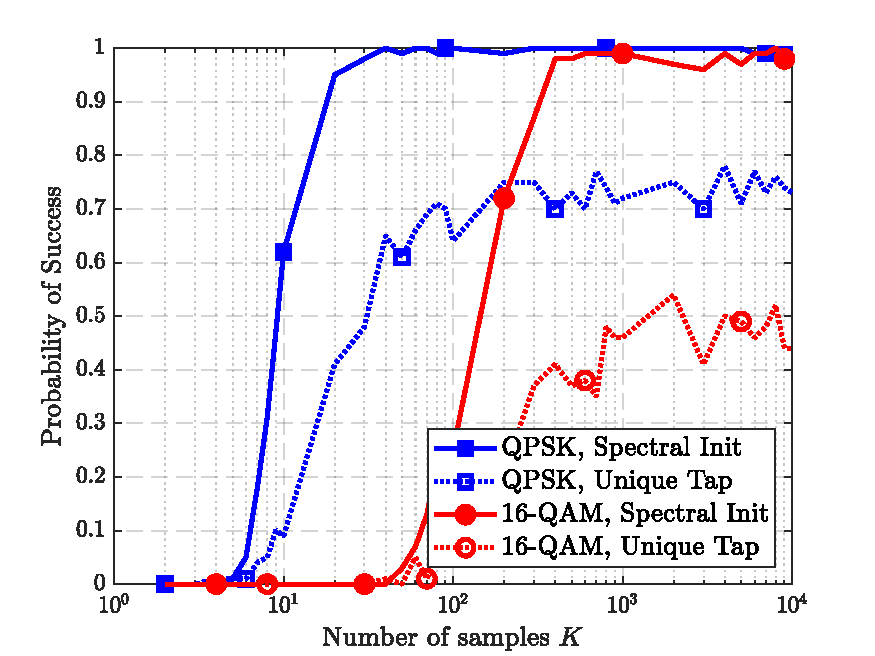
\includegraphics[width=\linewidth]{./figs/wfcma_figs/BF_WF_sucess_allmods_L=4_M=8_T=1000_mu=5e-4.pdf}	
	\subcaption{Success probability, $M=8,\,L=4$.}%Probability of successful recovery.}
\label{wfcma:fig:wf_ssr_success}
\end{subfigure}\hfill
\begin{subfigure}[t]{0.32\textwidth}
% Caption before figure
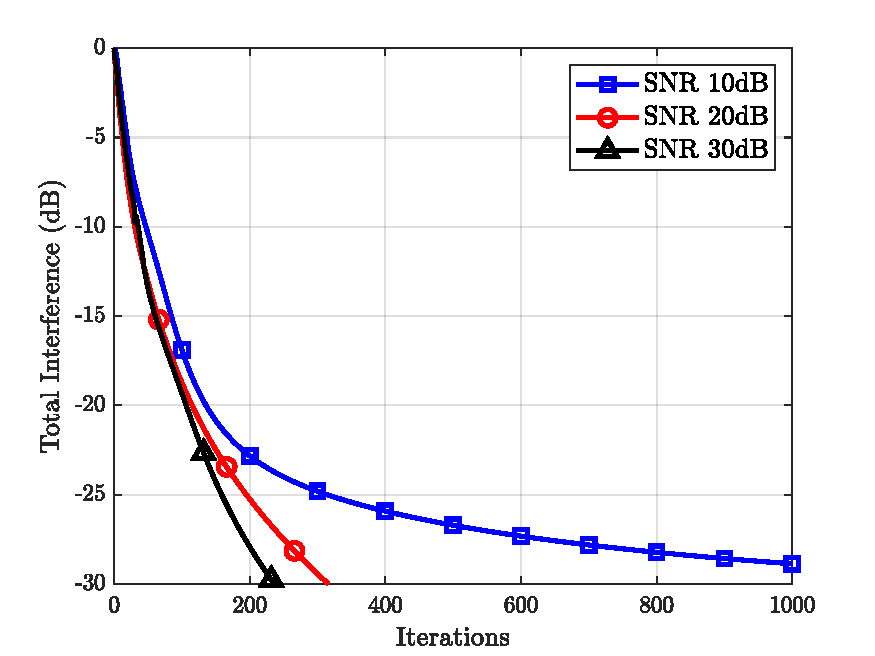
\includegraphics[width=\linewidth]{./figs/wfcma_figs/BF_WF_TI_4QAM_L=4_M=8_K=400_2.pdf}	
\subcaption{QPSK, $M=8,\,L=4$.}%Total Interference of QPSK, M=4,L=2.}
\label{wfcma:fig:wf_ssr_4qam_M8L4}
\end{subfigure}\hfill
\begin{subfigure}[t]{0.32\textwidth}
% Caption before figure
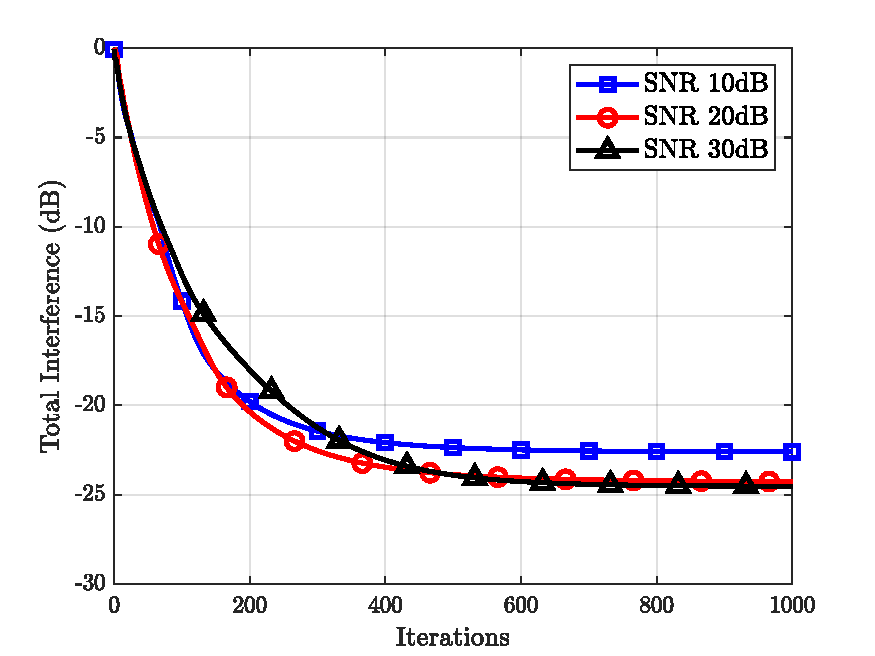
\includegraphics[width=\linewidth]{./figs/wfcma_figs/BF_WF_TI_16QAM_L=4_M=8_K=400_2.pdf}	
\subcaption{16-QAM, $M=8,\,L=4$.}%Total Interference of QPSK, M=8,L=4.}
\label{wfcma:fig:wf_ssr_16qam_M8L4}
\end{subfigure}\hfill
\\
\begin{subfigure}[t]{0.32\textwidth}
% Caption before figure
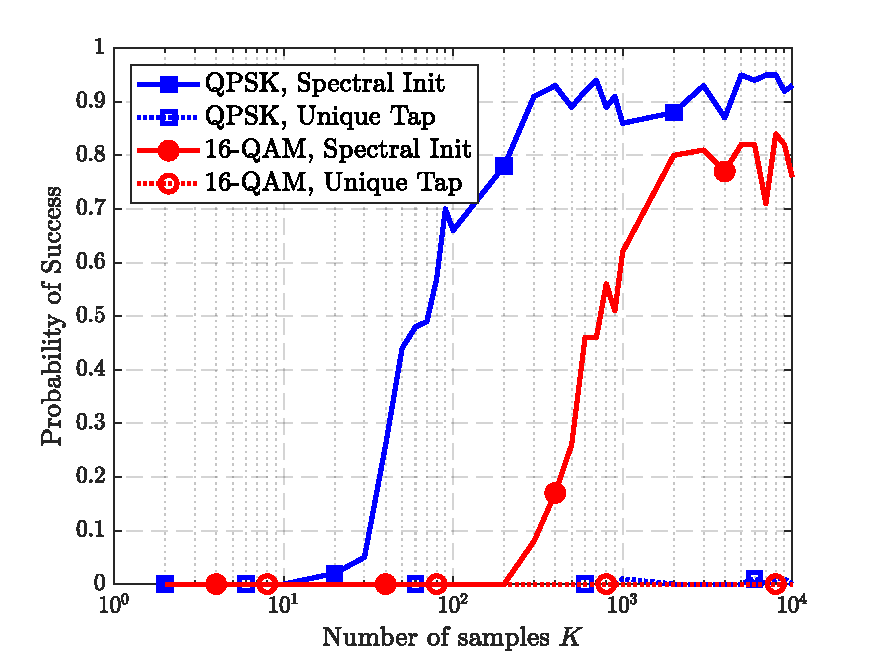
\includegraphics[width=\linewidth]{./figs/wfcma_figs/BF_WF_sucess_allmods_L=9_M=16_T=1000_mu=1e-4.pdf}	
\subcaption{Success probability, $M=16,\,L=9$.}%Total Interference of QPSK, M=8,L=4.}
\label{wfcma:fig:wf_ssr_success_M16L9}
\end{subfigure}\hfill
\begin{subfigure}[t]{0.32\textwidth}
% Caption before figure
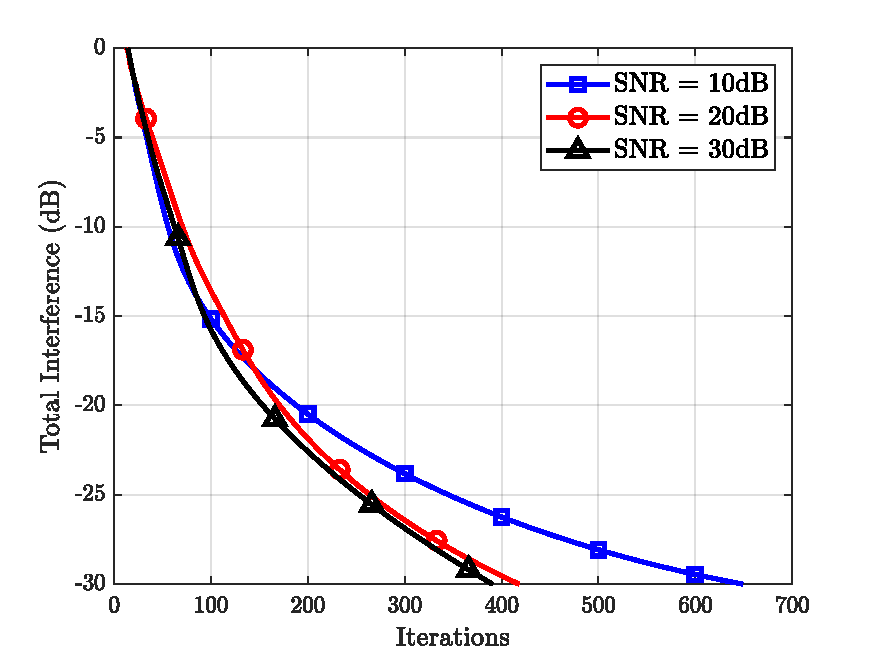
\includegraphics[width=\linewidth]{./figs/wfcma_figs/BF_WF_TI_4QAM_L=9_M=16_K=1000_2.pdf}
\subcaption{QPSK, $M=16,\,L=9$.}%Total Interference of 16QAM, M=4,L=2.}
\label{wfcma:fig:wf_ssr_4qam_M16L9}
\end{subfigure}\hfill
\begin{subfigure}[t]{0.32\textwidth}
% Caption before figure
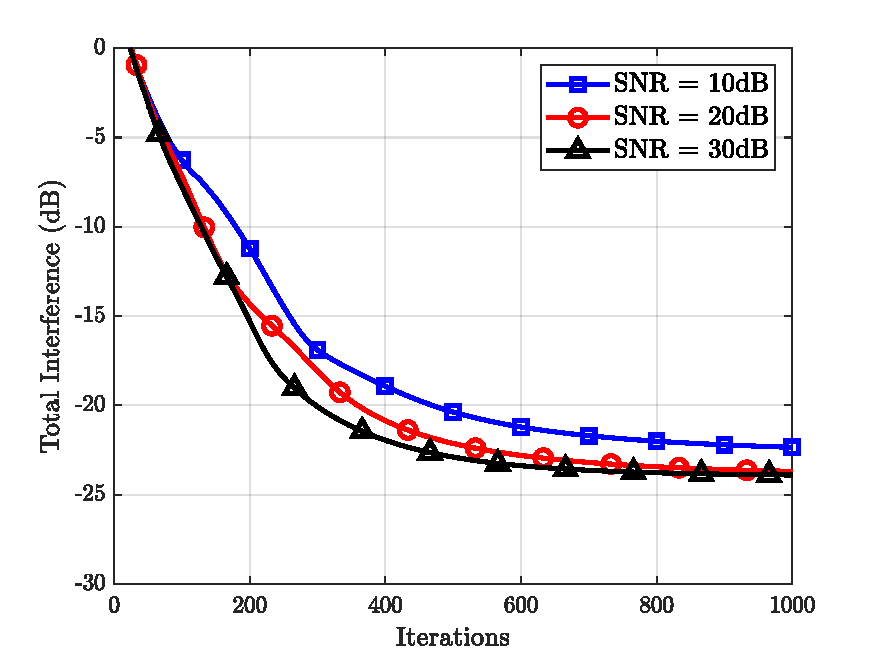
\includegraphics[width=\linewidth]{./figs/wfcma_figs/BF_WF_TI_16QAM_L=9_M=16_K=1000_2.pdf}	
\subcaption{16-QAM, $M=16,\,L=9$.}%Total Interference of 16QAM, M=8,L=4.}
\label{wfcma:fig:wf_ssr_16qam_M16L9}
\end{subfigure}
\caption{Numerical results of WF-CMA for single source recovery.}
\label{wfcma:fig:CMA_WF_ssr}
\end{figure*}

Figure~\ref{wfcma:fig:wf_ssr_success} presents the probability of successful recovery of a single source in a noiseless system with $L=4$ sources and $M=8$ receiving antennas.
We define ``success'' as the event of TISR reaching below $-20\,$dB after $T=1000$ iterations.
Two modulations (QPSK and 16-QAM) are tested. The results show that for QPSK, WF-CMA can actually converge to a solution even with a very small number of samples. 
For the higher-order modulation of 16-QAM, successful convergence requires about 10 times more data samples. 
More important, our test results show that spectral initialization of WF achieves better convergence than the traditional initialization that sets a random, unique tap of the demixer to 1 and others as 0. 
The higher probability of success achieved by spectral initialization empirically justifies its additional computational cost. 

Figure~\ref{wfcma:fig:wf_ssr_4qam_M8L4} illustrates the average TISR under QPSK modulation
under different SNR values. 
In this test, we used $K=400$ samples, $L=4$ sources and $M=8$ receiver antennas.
The results demonstrate desirable convergence with increasing number of iterations. 
On the other hand, 
Figure~\ref{wfcma:fig:wf_ssr_16qam_M8L4} shows the average TISR for 16-QAM modulation under the same test settings. 
For QPSK, the total interference to signal ratio can drop below $-27\,$dB even for $10\,$dB of SNR. 
For 16-QAM, the interference power remains several dB higher. Such results are expected for a
more complex modulation without constant modulus. Nevertheless, as shown in our analytical results,
the WF-CMA converges with the stepsize chosen according to Theorem~\ref{wfcma:thm:convergence_ssr}
and successfully suppresses multi-user interference. 

We repeat the experiments for a larger problem size of $L=9$ sources and $M=16$ receiver antennas.
Under similar conditions, the success probability of the WF-CMA under different sample sizes $K$ are also clearly shown in Figure~\ref{wfcma:fig:wf_ssr_success_M16L9}. These results further demonstrate the superior performance achieved using spectral initialization.
Correspondingly, the average TISR is shown in Figure~\ref{wfcma:fig:wf_ssr_4qam_M16L9} and Figure~\ref{wfcma:fig:wf_ssr_16qam_M16L9} for QPSK and 16-QAM, respectively. 
According to our analysis, we lowered the stepsize to $\mu=10^{-4}$ since the basin of attraction for size $\epsilon$ (depending on $B$) decreases with the number of sources $L$.
The resulting WF-CMA also shows successful recovery of a single source with sufficiently high interference suppression in for both QPSK and 16-QAM at different levels of SNR. 

\subsection{Multiple source recovery} \label{wfcma:sim:MSR} 

We now replicate the experiments above, attempting to simultaneously
recover $J=2$ sources at a time. We also set $\gamma_0=1$ and $\mu=1\cdot10^{-3}<2/\beta$ according to Theorem~\ref{wfcma:thm:convergence_msr}.

Figure~\ref{wfcma:fig:wf_msr_success} shows the probability of successful recovery of both sources given different numbers of samples in a noiseless system. 
We considered $L=4$ sources, $M=8$ receiving antennas for two different modulations of QPSK and 16-QAM. 
In the MSR case, success is defined as achieving less than $-20\,$dB TISR after $T=1000$ iterations in each demixer, both recovering distinct sources. 
Once again, the required number of samples for successful QPSK recovery appears quite small, whereas the number of samples required for successful 16-QAM recovery is approximately 10 times higher.

In Figure~\ref{wfcma:fig:wf_msr_4qam_M8L4} we show the average TISR of both demixers for QPSK signals under different levels of SNR.  
We let $K=400$ samples, $L=4$ sources and $M=8$ receiver antennas. 
Figure~\ref{wfcma:fig:wf_msr_16qam_M8L4} shows the achieved TISR for 16-QAM signals under the same setup. 
For QPSK source signals, the average TISR drops below $-30\,$dB for SNR of 20dB and 30dB within 400 iterations. 
For 16-QAM source signals,  the convergence rate is noticeably slower as 16-QAM constellation exhibits variable moduli.
\begin{figure*}
	\centering
	\begin{subfigure}[t]{0.32\textwidth}
		% Caption before figure
		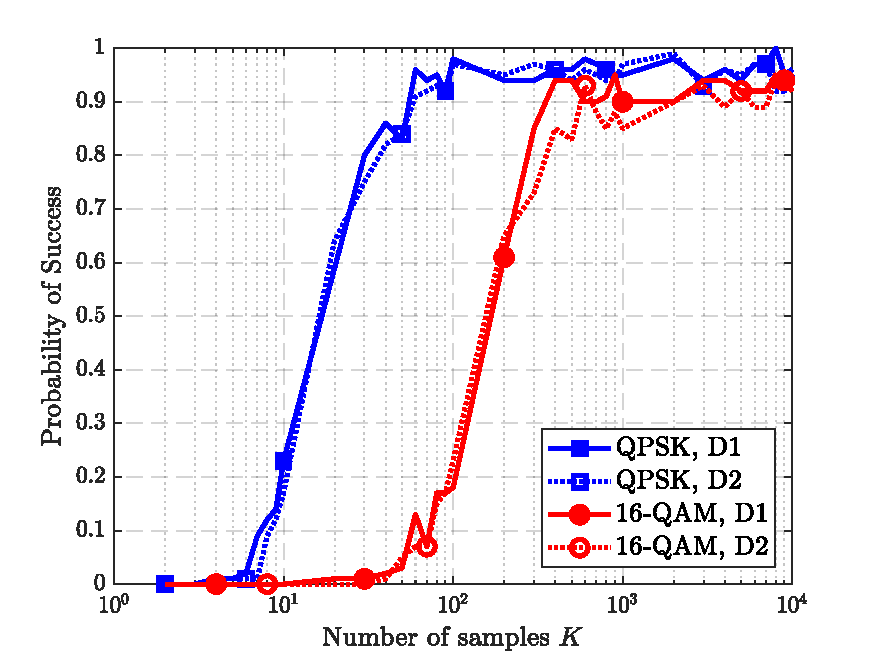
\includegraphics[width=\linewidth]{./figs/wfcma_figs/BF_WF_MSR_success_allmods_L=4_M=8_T=1000_mu=1e-3_gamma=1.pdf} 
		\subcaption{Success probability, $M=8,\,L=4$.}
		\label{wfcma:fig:wf_msr_success}
	\end{subfigure}\hfill
	\begin{subfigure}[t]{0.32\textwidth}
		% Caption before figure
		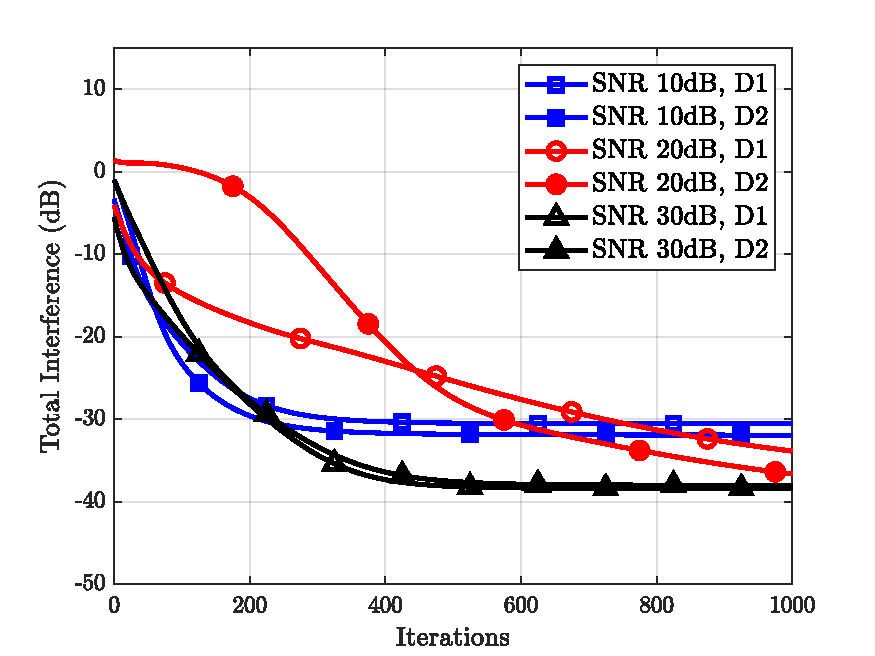
\includegraphics[width=\linewidth]{./figs/wfcma_figs/BF_WF_MSR_TI_4QAM_L=4_M=8_J=2_K=400_2.pdf}	
		\subcaption{QPSK, $M=4,\,L=8$.}
		\label{wfcma:fig:wf_msr_4qam_M8L4}
	\end{subfigure}\hfill
	\begin{subfigure}[t]{0.32\textwidth}
		% Caption before figure
		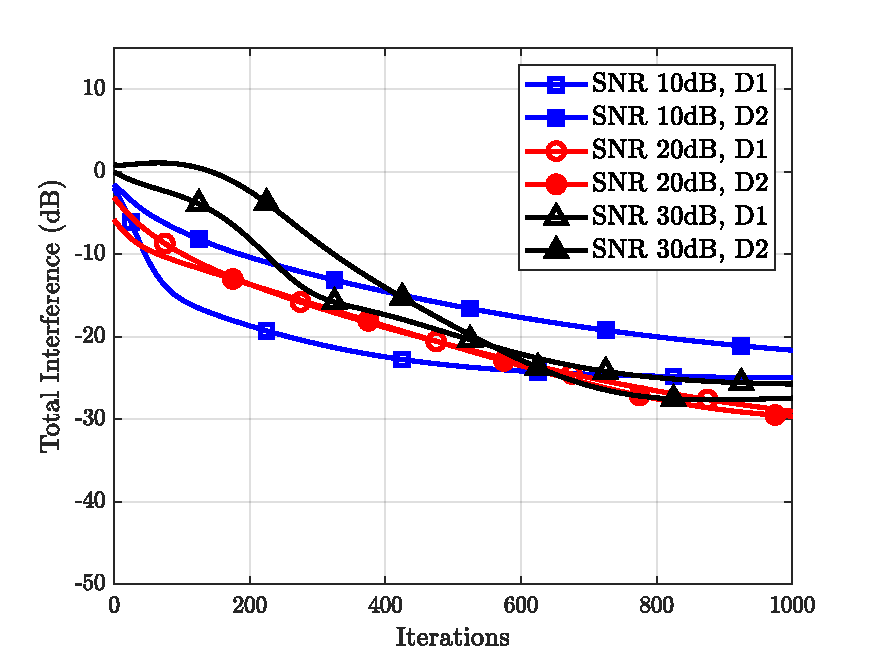
\includegraphics[width=\linewidth]{./figs/wfcma_figs/BF_WF_MSR_TI_16QAM_L=4_M=8_J=2_K=400_2.pdf}	
		\subcaption{16-QAM, $M=8,\,L=4$.}
		\label{wfcma:fig:wf_msr_16qam_M8L4}
	\end{subfigure}
	\\
	\begin{subfigure}[t]{0.32\textwidth}
		% Caption before figure
		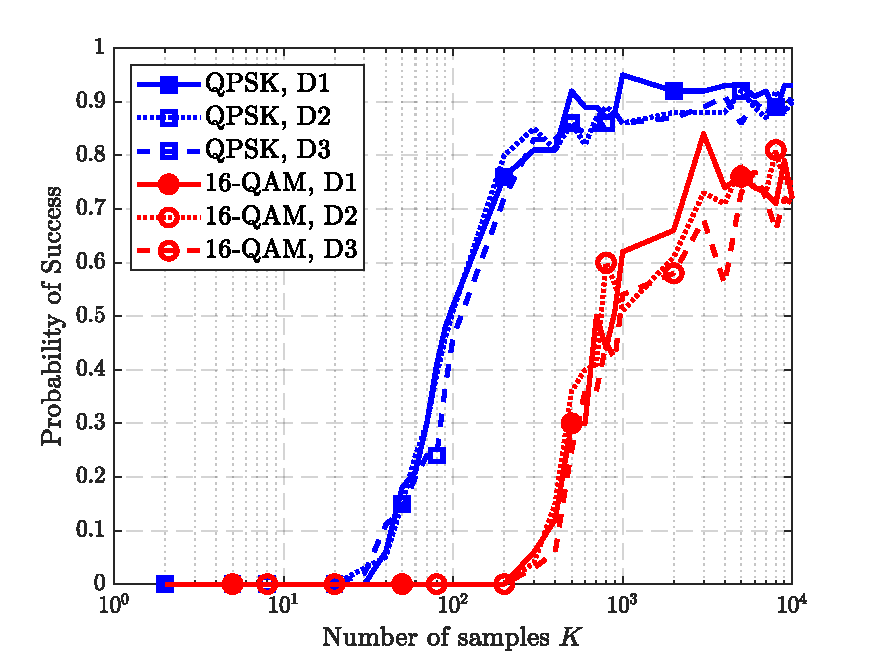
\includegraphics[width=\linewidth]{./figs/wfcma_figs/BF_WF_MSR_sucess_allmods_L=9_M=16_T=1000_mu=1e-4_gamma=1.pdf}
		\subcaption{Success probability, $M=16,\,L=9$.}
		\label{wfcma:fig:wf_msr_success_M16L9}
	\end{subfigure}\hfill
	\begin{subfigure}[t]{0.32\textwidth}
		% Caption before figure
		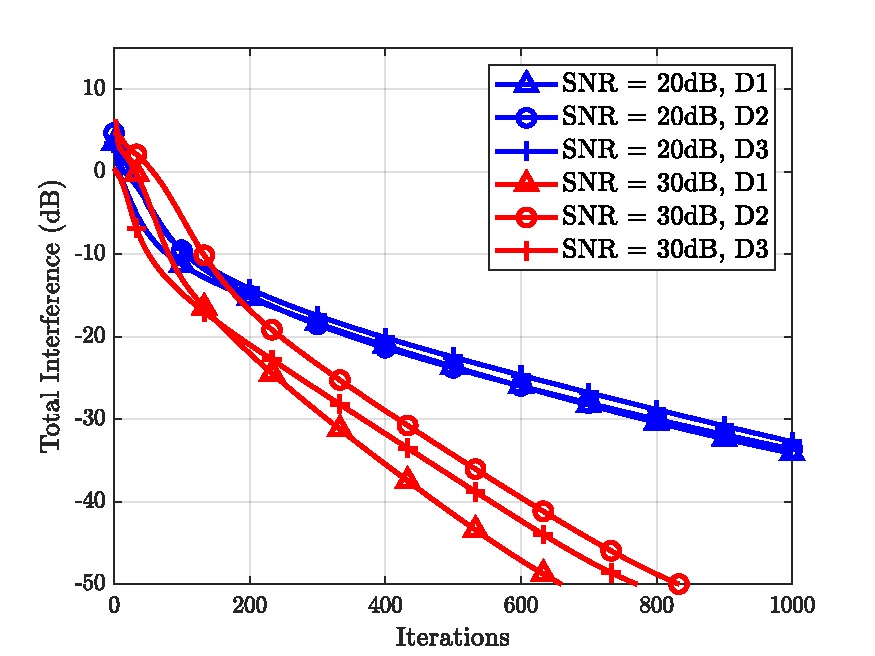
\includegraphics[width=\linewidth]{./figs/wfcma_figs/BF_WF_MSR_TI_4QAM_L=9_M=16_J=3_K=400_2.pdf}	
		\subcaption{QPSK, $M=16,\,L=9$.}
		\label{wfcma:fig:wf_msr_4qam_M16L9}
	\end{subfigure}\hfill
	\begin{subfigure}[t]{0.32\textwidth}
		% Caption before figure
		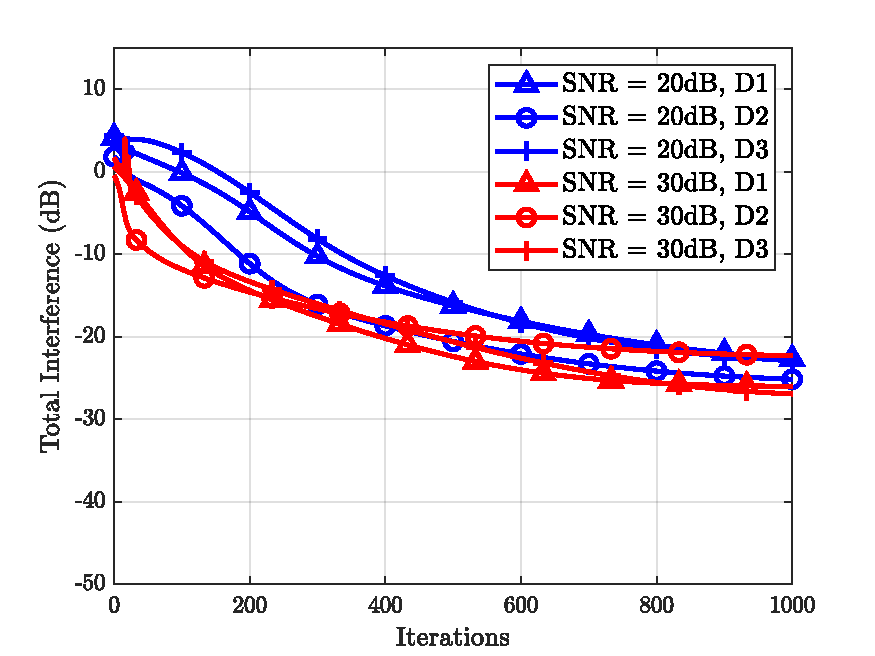
\includegraphics[width=\linewidth]{./figs/wfcma_figs/BF_WF_MSR_TI_16QAM_L=9_M=16_J=3_K=1000_2.pdf}	
		\subcaption{16-QAM, $M=16,\,L=9$.}
		\label{wfcma:fig:wf_msr_16qam_M16L9}
	\end{subfigure}
	\caption[Numerical results of WF-CMA for multiple source recovery.]{Numerical results of WF-CMA for multiple source recovery. We recover either $J=2$ or $J=3$ signals in each setting.}
	\label{wfcma:fig:CMA_WF_msr}
\end{figure*}

Next, we also consider the larger problem size with $L=9$ sources and $M=16$ receiver antennas. 
We use a stepsize of $\mu=10^{-4}$ for the same reasons explained in the single source recovery case. 
Figure~\ref{wfcma:fig:wf_msr_success_M16L9} shows the probability of successful recovery of both sources with
under $-20\,$dB TISR after 1000 iterations. The number of samples required for recovery increases with a larger system size, but not significantly. 
Figure~\ref{wfcma:fig:wf_msr_4qam_M16L9} and~Figure~\ref{wfcma:fig:wf_msr_16qam_M16L9} show the achieved average TISR for QPSK and 16-QAM sources, respectively. 
Both figures show that WF-CMA is able to recover two signals reliably at the same time.


\section{Summary}
In this chapter, we established a connection between Wirtinger Flow used in phase retrieval and CMA-based blind signal recovery in grant-free access. 
We generalized the convergence analysis of WF for our proposed algorithm by incorporating new conditions of subgaussian signal sources and average modulus, demonstrating its global convergence for blind signal recovery with high probability under limited data samples. 
We characterized the local geometry of the CM cost function in terms of local smoothness and convexity, which enables parameter updates to remain within the basin of attraction for a defined stepsize. Furthermore, we presented theoretical convergence guarantees for both single and multiple source recovery.
Our numerical tests demonstrated that our proposed algorithm can solve CMA-based blind signal recovery with a fast convergence rate and reasonable computational cost. 